\section{Introduction}
% what is ``Space subdivision''
Space Subdivision is the process of partitioning a space ($\mathcal{S}$), accroding to a provided set of level-curves\footnote{for simplicity, level-curves will be refered to as curves in the rest of the document.} ($\mathcal{C}$) in that space, into a set of faces ($\mathcal{F}$). 

\[ \mathit{subdivision}(\mathcal{S}, \mathcal{C}): \mathcal{S} \xrightarrow[]{decompose} \mathcal{F}\left(\mathcal{C}\right) \]

Figure~\ref{fig:intro_curvesPartitioning1} shows an example of a planar subdivision (where $\mathcal{S}$ is two dimensional), according to a set of curves containing six straight lines.
% what is it useful for? some application?
The process of subdivision provides an abstraction of the space.
Such an abstraction potentially facilitates the geometric processes required on that space.

\begin{figure}%[!ht]
  \centering
  \begin{subfigure}{.4\textwidth}
    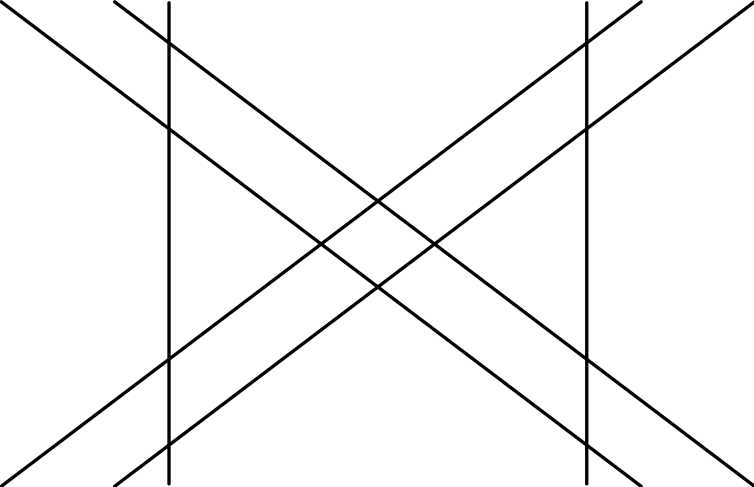
\includegraphics[width=\textwidth]{figures/intro_curves1.png}
    \caption{curves} \label{subfig:intro_curves1}
  \end{subfigure}%
  \quad \quad \quad%
  \begin{subfigure}{.4\textwidth}
    
\includegraphics[width=\textwidth]{figures/intro_partitioning1.png}
    \caption{partitionaing} \label{subfig:intro_partitioning1}
  \end{subfigure}%
  \caption[xxx]
          {A planar subdivision, over a set of curves containing six straight lines.
          Figure~\ref{subfig:intro_curves1} shows the set of curves, and the ``faces'' resulting from partitioning are color coded in figure~\ref{subfig:intro_partitioning1}.}
  \label{fig:intro_curvesPartitioning1}
\end{figure}

%%%%%%%%%%%%%%%%%%%%%%%%%%%%%%%%%%%%%%%%%%%%%%%%%%%%%%%%%%%%%%%%%%%%%%%%%%%%%%%%
\subsection{Problem Statement}

Here we define some of the terminologies, and breifly explain some of the challenges and requirements.

\paragraph{Curves}
A curve set $\mathcal{C}$ contians the level curves of some multivariable functions $f(X)$ defined over a space $\mathcal{S}$.
\[
\mathcal{C} = \lbrace c_i \mid c_i: f_i(X)=0, i \in I, \text{$I$: index set of $\mathcal{C}$} \rbrace
\]

\paragraph{Faces}
Every face is bounded to a closed curve and no curve crosses any face's surface.
%WIKI: a plane simple closed curve is a non-self-intersecting continuous loop in the plane (aka Jordan curve).
%WIKI: The Jordan curve theorem asserts that every Jordan curve divides the plane into an "interior" region bounded by the curve and an "exterior" region containing all of the nearby and far away exterior points,
The set of faces $\mathcal{F}$ satisfies following conditions:
\[
\begin{array}{l}
  \nexists f_i , f_j \in \mathcal{F}, \quad f_i \cap f_j \neq \emptyset \quad \text{($\cap$: geometric intersection)}\\
  \quad \\
  \displaystyle\bigcup_{ i \in \mathcal{I} } f_i \subseteq plane \quad \text{($I$: index set of $\mathcal{F}$)}
\end{array}
\]

\paragraph{Unbounded faces}
two approaches:
1) all unbounded faces are connected, i.e. any point out of the decomposition belong to the unbounded face.
2) unbounded faces are disconnect.
following the first approch, we treat the union of all unbounded faces as a single face.

\paragraph{Functionalities}
Membership and Neighborhood:

\[
\begin{array}{l}
  N\left(f_i\right) = \lbrace  f_j \mid \exists e_i, e_i \in f_i, e_i \in f_j \rbrace\\
  M\left(p\right) = f_i \quad \text{where point $p$ is inside $f_i$} \\
\end{array}
\]

%%%%%%%%%%%%%%%%%%%%%%%%%%%%%%%%%%%%%%%%%%%%%%%%%%%%%%%%%%%%%%%%%%%%%%%%%%%%%%%%
\subsection{Background}

Where the space $\mathcal{S}$ is two dimensional and the curve set $\mathcal{C}$ contians the level curves of only linear functions ($f(X)$).
\[
\mathcal{C} = \lbrace c_i \mid c_i: ax_1+bx_2+c=0, i \in I, \text{$I$: index set of $\mathcal{C}$} \rbrace
\]

Consequently every face is a polygone bounded to line segments.

%%%%%%%%%%%%%%%%%%%%%%%%%%%%%%%%%%%%%%%%
\subsubsection{Circles and the problem of non-convexity}

The first problem that rises from a non-convext region is, the expression of the region.
For instance the cross product won't work, therefore we need constraint-based description.

The circle in particular has a the circular behavior which means it is a closed (bounded) region.
Special case is where the circle resides inside a leaf, and with no intersection splits the leaf into sub-leaves.


%%%%%%%%%%%%%%%%%%%%%%%%%%%%%%%%%%%%%%%%%%%%%%%%%%%%%%%%%%%%%%%%%%%%%%%%%%%%%%%%
\subsection{This work}

\begin{figure}%[!ht]
  \centering
  \begin{subfigure}{.4\textwidth}
    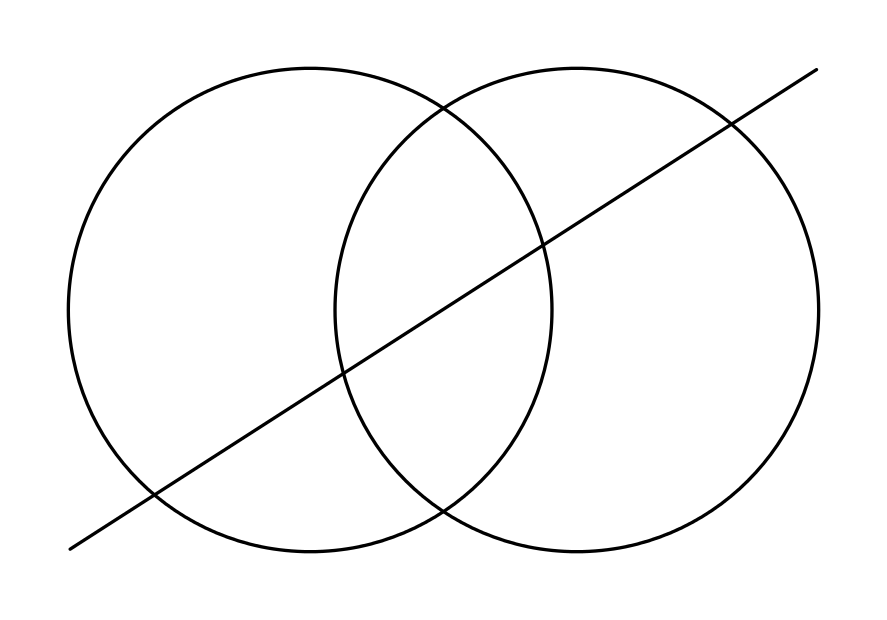
\includegraphics[width=\textwidth]{figures/intro_curves2.png}
    \caption{curves} \label{subfig:intro_curves2}
  \end{subfigure}%
  \quad \quad \quad%
  \begin{subfigure}{.4\textwidth}
    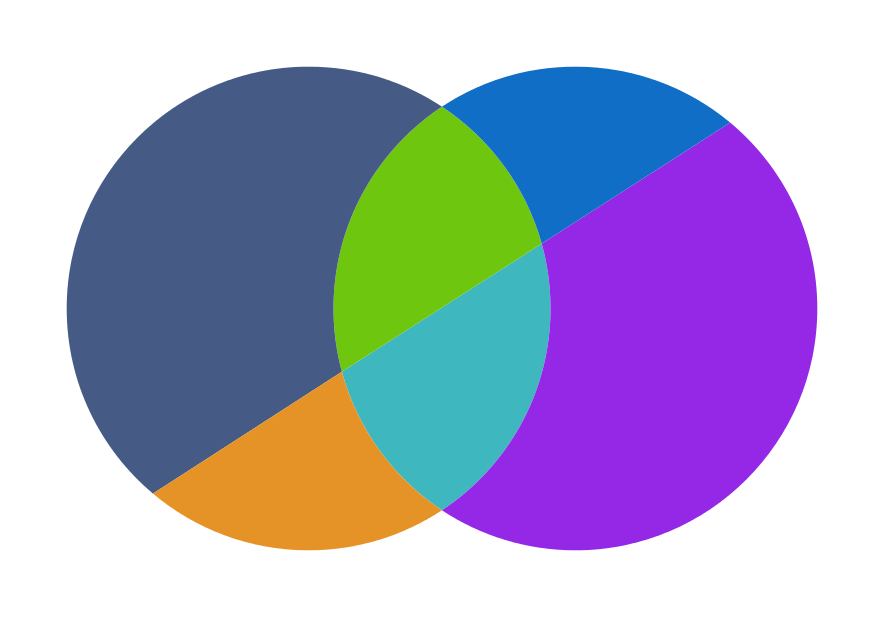
\includegraphics[width=\textwidth]{figures/intro_partitioning2.png}
    \caption{partitionaing} \label{subfig:intro_partitioning2}
  \end{subfigure}%
  \caption[xxx]
          {A planar subdivision, over a set of curves containing a straight line and two circles.
          Figure~\ref{subfig:intro_curves2} shows the set of curves, and the ``faces'' resulting from partitioning are color coded in figure~\ref{subfig:intro_partitioning2}.}
  \label{fig:intro_curvesPartitioning2}
\end{figure}

This work relies on the following assumptions:
\begin{description}
\item [Assumption 1] the space is a two dimensional plane.
\item [Assumption 2] if two curves were identical, their intersection would be the same curve which is beyond a finite set of points.
  in order to prevents the intersection procedure yielding a result other than a finite set of points,
  \[ \nexists c_i , c_j \in \mathcal{C}, \quad c_i = c_j \]
\item [Assumption 3] the set $\mathcal{C}$ contains levels curves resulted from either linear functions (straight lines as an example of an unbounded class) or conic sections (circles as an example of a bounded class).
\end{description}
